% L10c UCB1 figure: the upper confidence bounds of the lecture's worked example
% before round t = 6.
%
% Drawn on October 20, 2026 with the palette and build of the L10a figures.
%
% Each arm is a row on a reward scale (4.5 cm per unit reward). The dot is the
% arm's sample mean, and the bar extends by the confidence radius
% U(a, 6) = sqrt(2 log 6 / N_a) to the upper confidence bound. Values from the
% worked example:
%   arm 1: N_1 = 4, reward sum 3, mean 0.750, radius 0.947, bound 1.697
%   arm 2: N_2 = 1, reward sum 0, mean 0.000, radius 1.893, bound 1.893
% Arm 2 has the larger bound, so UCB1 pulls it in round 6. The dashed line is
% the largest possible reward, 1.
%
% Math uses the standard TeX fonts (no unicode-math), so symbols render as the
% notebook's math shows them.
%
% The notebook SVG carries a dark palette added by theme_svg.py; keep new
% colors in that script's mapping when changing the palette here.
\documentclass[tikz,border=4pt]{standalone}
\usepackage[no-math]{fontspec}
\IfFontExistsTF{Arial}{\setsansfont{Arial}}{\setsansfont{TeX Gyre Heros}}
\renewcommand{\familydefault}{\sfdefault}
\usepackage{amsmath,amssymb}

% Ink, blue, and gray match the L10a figures; blue marks the selected arm.
\definecolor{vnink}{HTML}{202124}
\definecolor{gdblue}{HTML}{0091FF}
\definecolor{gdgray}{HTML}{6D7278}

% \ucbrow{row y}{mean}{bound}{color}: the confidence bar of one arm, from its
% sample mean to its upper confidence bound, with an open dot at the mean.
\newcommand{\ucbrow}[4]{%
  \fill[#4] (4.5*#2, #1 - 0.11) rectangle (4.5*#3, #1 + 0.11);
  \draw[#4, line width=1.6pt] (4.5*#3, #1 - 0.24) -- (4.5*#3, #1 + 0.24);
  \filldraw[fill=white, draw=#4, line width=1.6pt] (4.5*#2, #1) circle (4pt);}

\begin{document}
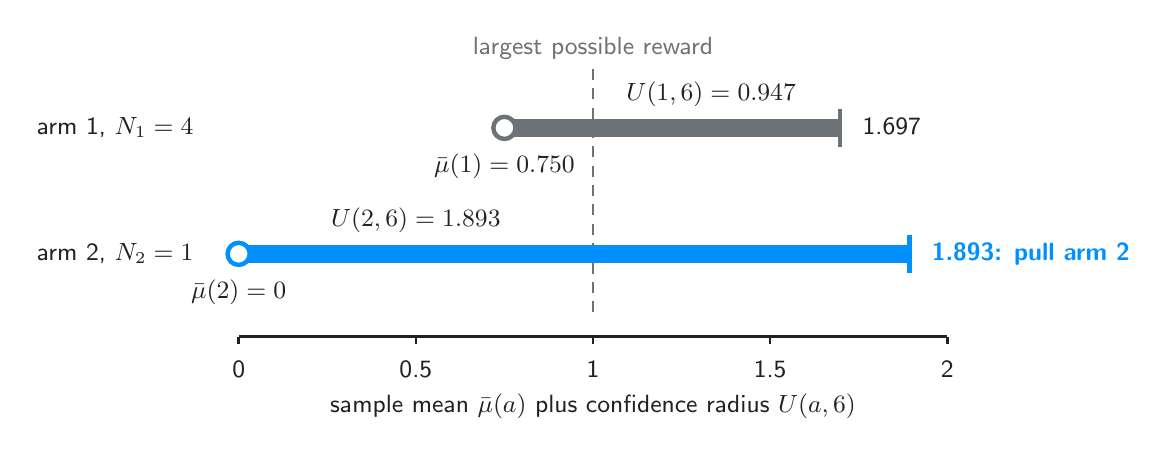
\begin{tikzpicture}[x=1cm, y=1cm, font=\sffamily\small, text=vnink,
    cell/.style={text height=1.6ex, text depth=0.45ex},
  ]
  % the largest possible reward
  \draw[gdgray, line width=0.8pt, dash pattern=on 4pt off 3pt] (4.5, 0.75) -- (4.5, -2.4);
  \node[anchor=south, text=gdgray] at (4.5, 0.75) {largest possible reward};

  % arm 1: four pulls, sample mean 0.75
  \ucbrow{0}{0.75}{1.697}{gdgray}
  \node[cell, anchor=east] at (-0.45, 0) {arm 1, $N_1=4$};
  \node[anchor=north] at (3.375, -0.2) {$\bar{\mu}(1)=0.750$};
  \node[anchor=south] at (6.0, 0.15) {$U(1,6)=0.947$};
  \node[cell, anchor=west] at (7.8, 0) {1.697};

  % arm 2: one pull, sample mean 0; the larger bound, so it is pulled next
  \ucbrow{-1.6}{0}{1.893}{gdblue}
  \node[cell, anchor=east] at (-0.45, -1.6) {arm 2, $N_2=1$};
  \node[anchor=north] at (0, -1.8) {$\bar{\mu}(2)=0$};
  \node[anchor=south] at (2.25, -1.45) {$U(2,6)=1.893$};
  \node[cell, anchor=west, text=gdblue, font=\sffamily\small\bfseries] at (8.68, -1.6) {1.893: pull arm 2};

  % reward scale
  \draw[vnink, line width=0.9pt] (0, -2.65) -- (9, -2.65);
  \foreach \v in {0, 0.5, 1, 1.5, 2} {
    \draw[vnink, line width=0.9pt] (4.5*\v, -2.65) -- (4.5*\v, -2.75);
    \node[cell, anchor=north] at (4.5*\v, -2.8) {\v};
  }
  \node[anchor=north] at (4.5, -3.25) {sample mean $\bar{\mu}(a)$ plus confidence radius $U(a,6)$};
\end{tikzpicture}
\end{document}
